\documentclass{article}

% Language setting
% Replace `english' with e.g. `spanish' to change the document language
\usepackage[spanish]{babel}

% Set page size and margins
% Replace `letterpaper' with `a4paper' for UK/EU standard size
\usepackage[letterpaper,top=2cm,bottom=2cm,left=3cm,right=3cm,marginparwidth=1.75cm]{geometry}

% Useful packages
\usepackage{ragged2e}
\usepackage{amsmath}
\usepackage{graphicx}
\usepackage{amssymb}
\usepackage[colorlinks=true, allcolors=blue]{hyperref}

\title {\textbf{El algoritmo de dos fases para el reconocimiento de actividades en el contexto de la Industria 4.0 y los procesos dirigidos por humanos
}}
\author{ Borja Bordel, Ramón Alcarria1, Diego Sánchez-de-Rivera1 1Universidad Politécnica de Madrid, Madrid, España bbordel@dit.upm.es, ramon.alcarria@upm.es, diegosanchez@dit.upm.es}

\begin{document}
\maketitle
\begin{abstract}
	Los futuros sistemas de industria, la revolución conocida como la Industria 4.0, están considerando integrar gente en el mundo de Internet como potenciales prosumidores (entre proveedores de servicios y consumidores). En este contexto, el trabajo dirigido por humanos aprece como una realidad esencial y los instrumentos para generar bucles  de información que se retroalimentan entre el subsistema social (personas) y el subsistema cibernético (componentes tecnológicas) son necesarios. A pesar de que muchos instrumentos distintos han sido propuestos, a día de hoy las técnicas de reconocimiento de patrones son las más prometedoras. Sin embargo, estas soluciones presentan algunos problemas pendientes. Por ejemplo, estos dependen del hadware seleccionado para obtener información de los usuarios; o presentan límites en el proceso de identificación. Para abordar esta situación, en este paper se propone un algoritmo de dos fases para integrar a las personas en los sistemas de la Industria 4.0. El algoritmo define acciones complejas como una composición de simples movimientos. Las acciones complejas son reconocidas utilizando los Movimientos Ocultos de Markov, y solo los movimientos simples se reconocen a través la DWT . De este modo, solo los movimientos dependen de los recursos de hadrdware empleados para capturar información, y se incrementa  la precisión en el reconocimiento de acciones complejas. Una validación experimental será también llevada a cabo para evaluar y comparar la interpretación de los resultados propuestos.
	Palabras clave: Industria 4.0; reconocimiento de patrones; DWT; Inteligencia Artificial; Modelos Ocultos de Markov.
\end{abstract}

\section{Introducción}
La Industria 4.0 [1] se basa en el uso sistemas Ciber-Físicos (uniones de procesos físicos y cibernéticos) [2] como componente tecnológica principal para futuras soluciones digitales, sobre todo  ( pero no únicamente) en el ámbito industrial. Por lo general, la digitalización ha causado, al final, el remplazo de los métodos tradicionales de trabajo por nuevos instrumentos digitales.
Por ejemplo, los trabajadores en producción en cadena fueron sustituidos por robots durante la tercera revolución industrial.
Sin embargo, algunas aplicaciones industriales no pueden basarse en soluciones tecnológicas, por lo que la mano de obra se vuelve esencial [3].  Los productos hechos a mano son un ejemplo que reflejan la importancia del trabajo humano. Estos sectores de la industria, en cualquier caso, deben integrarse en la cuarta revolución industrial. Desde la unión de los Sistemas Ciber-Físicos (CPS) y el papel de las personas como proveedores de servicios (trabajos activos), surgen los CPS humanizados[4]. En estos nuevos sistemas, los procesos dirigidos por humanos están permitidos; los procesos[5] i.e. que son conocidos, ejecutados y controlados por gente (aunque serán supervisados a través de mecanismos digitales).
Para una verdadera integración entre la gente y la tecnología, que elemine los procesos de ejecución humana o tecnológica, para lo que se requieren técnicas de extración de información. Durante los últimos años se han citado distintos métodos posibles, pero a día de hoy las técnicas de reconocimiento de patrones parecen las más promentedoras.
El uso de la IA, modelos estadísticos y recursos similares ha permitido un increíble desarrollo de los métodos de reconocimiento de patrones, aunque todavía quedan retos pendientes.
Inicialmente, las técnicas de reconocimiento de patrones dependen del hardware subyacente para la captura de información. La estructura y la memorización varía si (por ejemplo)   empleamos sensores de infrarrojos en vez de acelerómetros. Es muy problemática la velocicidad de evolución de las tecnologías hardware con respecto al software.
Por otro lado, existe un límite en la precisión del reconocimiento de procesos. De hecho, con las acciones humanas se vuelve más complicado, ya que se requieren más variables y modelos complejos para su reconocimiento. Esta aproximación genera grandes problemas de optimización con un error que aumenta al incrementar el número de variables, lo que provoca un decrecimiento del índice de reconocimiento[6]. En conclusión, las matemáticas (-------) aportan una cierta precisión al proceso de reconocimiento de patrones dando medidas para estudiar. Para evitar esta situación, deben ser consideradas menos variables. lo que reduce la complejidad del problema a la hora de analizarlo, una solución que no es aceptable en los ámbitos de la industria donde se desarrollan actividades de producción complejas.
Por lo tanto, el objetivo de este paper es describir un nuevo algoriitmo de reconocimiento de patrones dirigido a estos dos problrmas. El mecanismo propuesto define las acciones como una composición de movimientos simples. Estos se reconocen utilizando las técnicas de Deformación Dinámica del Tiempo (DTW) [7]. Este proceso depende del hardware empleado para la captura de información; pero las DTW son flexibles y la actualización del repositorio de reconocimiento es suficiente para configurar el algoritmo completo. Por otro lado, las acciones complejas son reconocidas como una combinación de movimientos simples a través de los Modelos Ocultos de Markov. HMM) [8]. Estos son totalmente independientes de la tecnología hardware , ya que solo consideran acciones simples. Estas dos fases  se aproximan y reducen la complejidad de los modelos, incrementando la precisión y el éxito del índice ene en el reconocimiento de patrones.
El resto del paper se organiza como sigue: en la Sección 2 se describe el funcionamiento del reconocimiento de patrones para actividades humanas; en la Sección 3 se describe la solución propuesta, incluyrndo las dos fases definidas; la Sección 4 presenta una prueba  experimental utilizando un escenario real; y la en la sección se concluye el paper.
\section {Estado del arte en el reconocimiento de patrones }
Se han informado muchas técnicas diferentes de reconocimiento de patrones para actividades humanas. Sin embargo, la propuesta más común puede clasificarse en cinco
categorías [9]: 
	(i) Modelos ocultos de Markov; 
	(ii) el campo aleatorio condicional de cadena de salto; 
	(iii) Patrones Emergentes; 
	(iv) el Campo Aleatorio Condicional; 
	(v) clasificadores bayesianos

De hecho, la mayoría de los autores proponen el uso de Modelos Ocultos de Markov (HMM) para modelar las actividades humanas. HMM permite modelar acciones como cadenas de Markov. Básicamente, HMM genera estados ocultos a partir de datos observables. En particular, el objetivo final de esta técnica es construir la secuencia de estados ocultos que encaje con una determinada secuencia de datos. Para finalmente definir todo el modelo, HMM debe deducir de los datos los parámetros del modelo de manera confiable. La figura 1 muestra una representación esquemática de cómo funciona HMM. Cuando se reconocen las actividades humanas, las acciones que componen las actividades son los estados ocultos y las salidas de los sensores son los datos que se estudian. HMM, además, permite el uso de técnicas de entrenamiento considerando el conocimiento previo sobre el modelo. Este entrenamiento a veces es esencial para “inducir” todas las posibles secuencias de datos requeridas para calcular el HMM. Finalmente, es muy importante tener en cuenta que los HMM aislados simples se pueden combinar para crear modelos más grandes y complejos.

\begin{figure}[h]
\centering
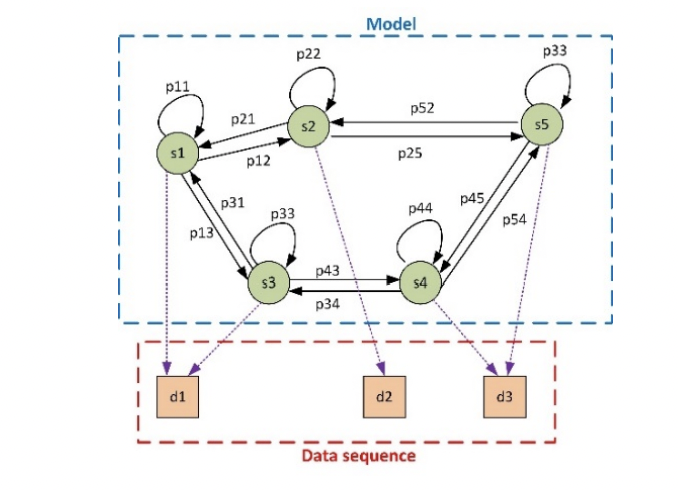
\includegraphics[width=0.3\textwidth]{punto2.png}
\caption{\label{fig:frog}Representación gráfica de un HMM .}
\end{figure}

Los HMM, sin embargo, son inútiles para modelar ciertas actividades concurrentes, por lo que otros autores han reportado una nueva técnica denominada Conditional Random Field (CRF). Los CRF se emplean para modelar aquellas actividades que presentan acciones concurrentes o, en general, múltiples acciones que interactúa. Además, HMM requiere un gran esfuerzo de entrenamiento para descubrir todos los estados ocultos posibles. Para resolver estos problemas, el campo aleatorio condicional (CRF) emplea probabilidades condicionales en lugar de distribuciones de probabilidad conjunta. De esa forma, se pueden modelar fácilmente actividades cuyas acciones se desarrollan en cualquier orden. A diferencia de las cadenas en HMM, CRF emplea gráficos acíclicos y permite la integración de estados ocultos condicionales (estados que dependen de observaciones pasadas y/o futuras).
Los CRF, por otro lado, siguen siendo inútiles para modelar ciertos comportamientos, por lo que algunas propuestas generalizan este concepto y proponen el Skip Chain Conditional Random Field (SCCRF). SCCRF es una técnica de reconocimiento de patrones, más general que CRF, que permite modelar actividades que no son una secuencia de acciones en la naturaleza [14]. Esta técnica trata de capturar dependencias de largo alcance (cadena de salto); y puede entenderse como el producto de diferentes cadenas lineales. Sin embargo, al calcular este producto
es bastante pesado y complicado, por lo que esta técnica suele ser demasiado costosa desde el punto de vista computacional para implementarla en pequeños sistemas integrados.
Otras propuestas emplean técnicas de descripción de mayor nivel como Emerging Patterns (EP). Para la mayoría de los autores, EP es una técnica que describe actividades como vectores de parámetros y sus valores correspondientes (ubicación, objeto, etc.).  Utilizando distancias entre vectores es posible calcular y reconocer acciones desarrolladas por personas. Finalmente, otros autores han empleado con éxito técnicas secundarias como los clasificadores bayesianos, que identifican actividades haciendo una correspondencia entre las actividades humanas y las salidas más probables de los sensores mientras se realizan estas acciones, considerando que todos los sensores son independientes. Los árboles de decisión, las extensiones HMM y otras tecnologías similares también se han estudiado en la literatura, aunque estas propuestas son escasas.
Entre todas las tecnologías descritas, HMM no es la más poderosa. Sin embargo, encaja a la perfección con la Industria 4.0, donde las actuaciones son muy complejas pero muy estructuradas y ordenadas (según protocolos de empresa, políticas de eficiencia, etc.). Además, se requiere una retroalimentación rápida (a veces incluso en tiempo real) para garantizar que los procesos impulsados por humanos funcionen correctamente antes de que ocurra una falla crítica global. Por lo tanto, las soluciones computacionalmente costosas no son un enfoque válido, y estamos seleccionando HMM como tecnología de base principal. Para preservar su carácter liviano y, al mismo tiempo, poder modelar actividades complejas, introducimos un esquema de reconocimiento de dos fases que permite dividir acciones complejas en dos pasos más simples.
\section {Algoritmo de reconocimiento de patrones en dos fases}

Con el fin de (i) independizar el proceso de reconocimiento de patrones de usar aparatos de hardware para capturar información, (ii) permitir el reconocimiento de movimientos complejos, y (iii) preservar el carácter ligero de los modelos seleccionados, la solución propuesta una arquitectura con 3 capas tal que:


\begin{figure}[h]
\centering
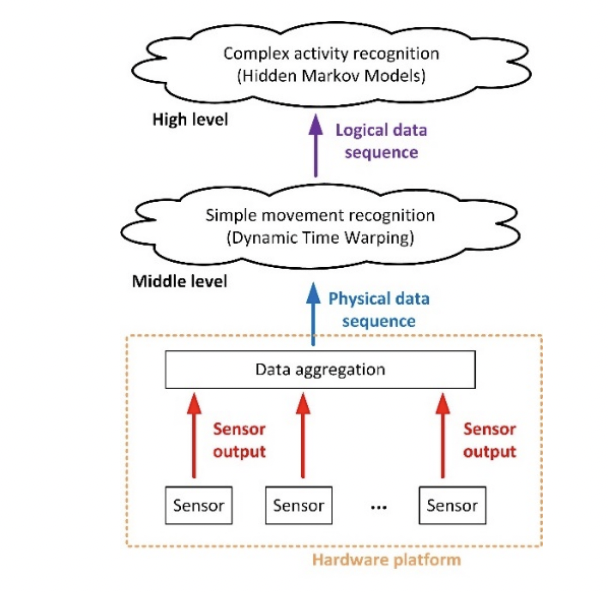
\includegraphics[width=0.3\textwidth]{punto3.png}
\caption{\label{fig:frog}Arquitectura de la solución propuesta del patrón de reconocimiento.}
\end{figure}

La capa más baja incluye la plataforma de hardware. Dispositivos de vigilancia como
acelerómetros, teléfonos, sensores infrarrojos, etiquetas RFID, etc., se implementan para
capturar información sobre el comportamiento de las personas. Las salidas de estos dispositivos crean
secuencias de datos físicos cuyo formato, rango dinámico, etc., dependen totalmente de
las tecnologías de hardware seleccionadas.

Estas secuencias de datos físicos luego se procesan en la capa intermedia usando tecnicas de DTW. Como resultado, para cada secuencia de datos físicos, un simple movimiento o acción es reconocido. Estos movimientos simples se representan usando un formato de datos binarios para hacer la solución lo menos pesada posible. El software de este nivel debe modificarse cada vez que se actualiza la plataforma de hardware, pero las tecnologías DTW no requieren de un gran proceso de actualización, y actualizar el repositorio de patrones es suficiente para configurar el
algoritmo en este nivel.

Los movimientos simples reconocidos se agrupan para crear secuencias de datos lógicos. Estas secuencias alimentan un sistema de reconocimiento de patrones de alto nivel basado en los modelos ocultos de Markov. En este nivel, los componentes de software requieren un fuerte proceso de entrenamiento, pero la capa intermedia hace totalmente independiente la plataforma de hardware y de modelos de alto nivel. Por lo tanto, cualquier cambio en la plataforma de hardware no impone una actualización en el HMM, lo que sería extremadamente costoso computacionalmente. Por el análisis de
la secuencia de movimientos simples, se reconocen acciones complejas.
La siguiente subsección describe en detalle las dos fases de reconocimiento de patrones propuestas.

\subsection{Reconocimiento de movimientos simples: Dinámicas de Deformación del Tiempo}
Para reconocer gestos o movimientos simples, se han seleccionado las técnicas de Deformación Dinámica del Tiempo. Estas tecnologías cumplen con los requisitos de los componentes de software de nivel medio, ya que se adaptan muy bien a las características de la plataforma de hardware facilmente y son más rápidas y eficientes.(así los aparatos instegrados las implementan).
En nuestra solución, el comportamiento humano se motriza a través de la familia de sensores simbolo S, conteniendo las Ns componentes (1).


Las salidas de estos sensores se muestran periódicamente como Ts: obteniendo para cada instante de tiempo, t, un vector de  Ns valores (cada valor de cada sensor). Este vector  Yt se llama “muestra multidimensional simple” (2).


Después, un movimiento simple Y tendrá una duración de  Tm  segundos y se describirápor la secuencia temporal de Nm muestras multidimensionales recogidas durante ese tiempo (3). Para el reconocimiento de movimientos tardíos, se crea un repositorio de patrón símbolo R que contienen las secuencias temporales correspondientes para cada una de las acciones simples de K para reconocerlas (4). 


Por lo general,la gente realiza movimientos de un modo similar pero diferente. Por esto, las transicioens deben ser lentas o rápidas, algunas acciones elementales deben ser añadidas o eliminadas etc. Por lo tanto, dando una secuencia X  Nx muestras, representando un movimiento para ser reconocido,deben estar localizadas en el patrón  Ri ⋲ simbolo R mas cercano a X; por lo que Ri se reconoce como una acción realizada. Para hacer esto se define la función distancia (5). Esta función que se aplica para calcular el valor de la matriz, necesitamuestras que muchas veces no tienen la misma longitud ni están alineadas(6).

En los sensores de posición (acelerómetros, aparatos de infrarrojos, etc) la función distancia es directamente aplicada a los sensores de salida (lo contrario ocurre, por ejemplo, en los micrófonos donde las salidas deben ser evaluadas en la carga deldominio). Aunque también pueden utilizarse otras funciones distancia (La divergencia simétrica de Kullbabk-Leibler o la distacncia Manhattan), para este primer trabajo se utilizan las distancias Euclideas estándar (7).


Después, se define la ruta de deformación p = (p1,p2…pL) como una secuencia de pares (nl, ml) con (nl, ml) ⋲ [1,Nx]X[1,Nm] y l ⋲ [1,L], satisfaciendo las trés condiciones: (i) el límite, i.e. p1= [1,1] y pL =[Nx,Nm];(ii) la monotonía , i.e. n1≤n2...≤nL y m1≤m2≤…≤mL; y (iii) la condición de intensidad de paso i.e. pl-p(l-1) ⋲ {(1,0), (0,1), (1,1)} con l⋲[1, L-1].
Luego, el valor total de la ruta pi se calcula añadiendo todos los valores o distancias parciales (8). Con todo esto, la distancia entre dos secuencias de datos Ri y X se define como el valor (distancia) da la ruta más óptima (9).

Finalmente, el movimiento simple es reconocidopor la secuencia de datos X que es el que tiene el patrón Ri menor distancia (el más cercano) a X. Esta descripción es transigente con las variaciones de velocidad en la ejecución de movimientos, la intreoducción de nuevos microgestos, etc. Además,como se puede ver, cuando un hardware diferente se desplega, esto basta para actualizar el repositorio de la ruta simbolo R para reconfigurar toda la solución al patrón de reconocimiento ( ya que no se requiere entrenamiento).

\subsection{Reconocimiento de movimientos complejos: Modelos Ocultos de Markov}

El mecanismo propuesto anteriormente es muy útil para reconocer acciones simples, pero las actividades complejas involucran una gran cantidad de variables y requieren mucho más tiempo.
Por lo tanto, DTW tiende a volverse impreciso y se requieren modelos probabilísticos. Entre todos los modelos existentes, HMM es el más adecuado para escenarios industriales y procesos humanos.

De la fase anterior, la infinidad de posibles movimientos simples de ser reconocidos es $\mathcal{M} =  \left\lbrace \ m_i,\ i=1,\cdots , \ K \right\rbrace$. Además, se define un universo de estados  $\mathcal{U} =  \left\lbrace \ u_i,\ i=1,\cdots , \ Q \right\rbrace$, describiendo todos los estados que las personas pueden atravesar mientras interpretan cualquier acción bajo un estudio previo.



Entonces, una serie de observaciones $\mathcal{O} =  \left\lbrace \ o_i,\ i=1,\cdots , \ Z_o \right\rbrace$ (movimientos simples reconocidos en la fase anterior) han sido consideradas, además de la secuencia de estados  $\mathcal{S} =  \left\lbrace \ s_i,\ i=1,\cdots , \ N_s \right\rbrace$ describiendo la acción para ser modelada por HMM. En este caso inicial, asumimos cada observación correspondiente a un nuevo estado, asi que  $\mathcal{S} =  \left\lbrace \ s_i,\ i=1,\cdots , \ N_s \right\rbrace$. Entonces, 3 matrices son calculadas: (i) la matriz transitoria A (10) describiendo la probabilidad del estado(uj) siguiendo el estado (ui); (ii) la matriz de observación (11) describiendo la probabilidad de observación(oj) causada por el estado (uj) independientemente de k; y (iii) la matriz de probabilidad inicial(12).

\begin{equation}A  =\left[a_\imath ,\jmath \right] \ \ a\imath ,\jmath = P\left(v_k = u\jmath \ | \ v_k-1 = u\imath  \right)\end{equation}

\begin{equation}B  =\left[b_\jmath \left(o_\imath \right)  \right] \ \ b_\jmath \left(o_\imath \right)  = P\left(x_k = o_\imath | v_k = u_\jmath  \right)  \end{equation}

\begin{equation}\prod =\left[\pi_\imath \right] \ \ \pi_\imath = P\left(v_1= u_1\right)  \end{equation}

Entonces, el HMM para cada actividad compleja(landai) para ser reconocida se describe gracias a estos 3 elementos previos(13).
\begin{equation}\lambda i=\left\{A\imath ,B_\jmath ,\prod_i  \right\}\end{equation}

Además, se hacen dos supuestos: (i) el de Markov(14) mostrando que cualquier estado depende solo del anterior; y (15) el de independencia, afirmando que cualquier secuencia de observación depende sólo del estado presente, no de estados previos u observaciones.


\begin{equation} P\left(v_k | v_1, ... , v_{k-1}\right) \ = \ P\left(v_k \ | \ v_{k-1}\right)  \end{equation}

\begin{equation}P\left(o_k \ | \ o_1, ..., o_{k-1}, v_1,...,v_k\right) = P\left(o_k \ | \  v_k\right)\end{equation}

Para evaluar el modelo y reconocer la actividad que están realizando los usuarios, en este papel estamos utilizando un enfoque tradicional(16). Aunque los algoritmos directos han demostrado ser más eficientes, para este trabajo inicial estamos implementando directamente la expresión de evaluación en su forma tradicional.

16

El proceso de aprendizaje también se implementó en su forma más sencilla. Estadístico se emplearon definiciones para matriz transitoria, matriz de observación y matriz inicial.
matriz de probabilidad. En particular, se empleó la definición de probabilidad de Laplace estimar estas tres matrices a partir de estadísticas sobre las actividades en estudio(17-19). El símbolo(·) indica el número de veces que ocurre.

\begin{equation} a_{\imath\jmath}  = P\left(u_\jmath  | u_\imath \right) = \frac{contar\left(u_\jmath \ seguido \ de \ u_\imath  \right) }{contar\left(u_\jmath \right) } \end{equation}

\begin{equation}b_\jmath\left(o_\imath \right) = P\left(o_i \ | \ u_\jmath \right)  = \frac{contar\left(o_\imath \ esta \ observado \  en \  el \  estado \ u_\jmath \right) }{contar\left(u_\jmath \right) }  \end{equation}

\begin{equation}\pi_\imath  = P\left(v_1 = u_\imath \right) = \frac{contar \ \left(v_1 = u_\imath \right)  }{contar\left(v_1\right) }  \end{equation}

\section {Validación experimental: implementación y resultados}
Con el fin de evaluar el cumplimiento de la solución propuesta, se ha designado una validación experimental y se ha llevado a cabo. Un escenario industrial ha sido imitado en algunas salas grandes de la Universidad Politécnica de Madrid. El escenario representó a una compañia tradicional de producción de productos hechos a mano. En particular, imitaron un pequeño PCB(placa de circuito impreso) productor.

Para conseguir información sobre el comportamiento de las personas, a varios participantes se les proporcionó guantes cibernéticos, incluyendo acelerómetros y un lector RFID. Los objetos cercanos al escenario fueron identificados con una etiqueta RFID, por lo que la plataforma de hardware propuesta puede identificar la posición de la mano y los objetos con los que las personas han interactuado.

Una lista de 12 actividades diferentes fue diseñada y definida usando la tecnología propuesta. La tabla 1 describe las 12 actividades definidas, además de una breve descripción sobre ellas. 

\begin{table}[h]
	\begin{center}
		\begin{tabular}{ | p{4cm} | p{9cm} | }
			\hline Actividad                                   & Descripción                                                                                                              \\ \hline
			Dibujar las rutas de los circuitos                 & El circuito para ser impreso es diseñado usando un programa PC de software específico                                    \\ \hline
			Imprimir el circuito diseñado usando un plóter     & Usando fundas externas y un plóter, el circuito diseñado es impreso                                                      \\ \hline
			Limpiar las caras del laminado de cobre            & Usando un producto especial, todo el polvo y las partículas se eliminan de las caras del laminado de cobre               \\ \hline
			Copiar el circuito diseñado en las caras del cobre & El circuito diseñado en las fundas externas se copia en el laminado de cobre usando una explosión de rayos ultravioletas \\ \hline
			Sumergir las placas en la piscina con ácido        & Para eliminar lo innecesario del cobre, sumergimos las caras del laminado de cobre en un baño de ácido                   \\ \hline
			Lavar el cobre con un baño de disolvente           & Después del baño de ácido, la superficie del cobre restante se lava con un baño de disolvente                            \\ \hline
			Capa de alineamiento                               & PCB están compuesto de varias capas, alineadas y amontonadas durante su fase                                             \\ \hline
			Inspección óptica                                  & Se revisa la capa de alineamiento con un láser                                                                           \\ \hline
			Unir las capas exteriores con el sustrato          & Usando un pegamento epóxico, las capas finales y exteriores de las placas se unen                                        \\ \hline
			Unir la placa                                      & La unión ocurre en una mesa de acero pesado con abrazaderas metálicas                                                    \\ \hline
			Taladrar los agujeros necesarios                   & Los agujeros para componentes, etcétecera, son taladrados en el montón de placas                                         \\ \hline
			Enchapado                                          & En un horno, la placa está lista                                                                                         \\ \hline
		\end{tabular}
	\end{center}
\caption{\label{fig:frog}Tasa media de éxito para la solución propuesta.}
\end{table}


18 personas estuvieron involucradas en el experimento. Las personas fueron solicitadas para realizar las actividades con números aleatorios. El orden verdadero, así como el de las actividades es reconocido y almacenado por un proceso de software supervisor. La tasa global de éxito para todas las soluciones ha sido evaluada, identificando, el mismo éxito para cada una de las distintas fases.

Para evaluar las mejoras obtenidas en comparación con las soluciones similares ya existentes, la misma secuencia de datos físicos ha sido empleada para alimentar la solución de un patrón estándar de reconocimiento basado solo en HMM. Usando un software de procesamiento de datos específicos, algunos resultados relevantes han sido obtenidos.

La figura 4 representa la tasa media de éxito para 3 casos: la solución global, la primera fase(DTW) y la segunda fase (HMM). Además, la tasa de éxito para el tradicional HMM-based acercamiento está incluido. Como se puede ver, la tecnología sugerida es, globalmente, alrededor de un 9 \% mejor que  las técnicas tradicionales de reconocimiento de patrón basadas en HMM exclusivamente. Además, la primera fase(basada en DTW) es alrededor de un 20 \% peor que la segunda fase(HMM) que es significativo que las DTW técnicas son más débiles por defecto.


\section {Conclusiones y futuros trabajos}
En este paper presentamos un nuevo patrón algorítmico de reconocimiento para integrar individuos en los sistemas de la Industria 4.0 y los procesos dirigidos por humano. El algoritmo define actividades complejas como una composición de movimientos simples. Las actividades complejas son reconocidas empleando los Modelos Ocultos de Maekov, y los movimientos simples son reconocidos utilizando las DWT. Con el fin de activar el implemento de este algoritmo incrustado en objetos pequeños, se seleccionan configuraciones ligeras. Una prueba experimental de esto es llevarlo a cabo, y los resultados muestran una mejora global en un exitoso índice del 9%.
Los futuros trabajos considerarán metodologías más complejas para el procesamiento de datos, y la comparación para configuraciones distintas de la propuesta serán evaluadas.
Además, la propuesta será analizada en diferentes escenarios.




\end{document}